\documentclass[conference]{IEEEtran}
\IEEEoverridecommandlockouts

\usepackage{listings}
% Define slightly more reasonable Listings defaults
\lstset{
    basicstyle=\ttfamily\small,
    breaklines=true,
    prebreak=\raisebox{0ex}[0ex][0ex]{\ensuremath{\hookleftarrow}},
    frame=lines,
    showtabs=false,
    showspaces=false,
    showstringspaces=false,
    keywordstyle=\color[gray]{0.4}\bfseries,
    commentstyle=\color[gray]{0.65}\itshape,
    numbers=left,
    captionpos=b,
}
\usepackage{color}
\usepackage{fancyvrb}
\usepackage{fvextra}
\newcommand{\VerbBar}{|}
\newcommand{\VERB}{\Verb[commandchars=\\\{\}]}
\DefineVerbatimEnvironment{Highlighting}{Verbatim}{commandchars=\\\{\}, breaklines=true}
% Add ',fontsize=\small' for more characters per line
\newenvironment{Shaded}{}{}
\newcommand{\KeywordTok}[1]{\textcolor[rgb]{0.00,0.44,0.13}{\textbf{{#1}}}}
\newcommand{\DataTypeTok}[1]{\textcolor[rgb]{0.56,0.13,0.00}{{#1}}}
\newcommand{\DecValTok}[1]{\textcolor[rgb]{0.25,0.63,0.44}{{#1}}}
\newcommand{\BaseNTok}[1]{\textcolor[rgb]{0.25,0.63,0.44}{{#1}}}
\newcommand{\FloatTok}[1]{\textcolor[rgb]{0.25,0.63,0.44}{{#1}}}
\newcommand{\CharTok}[1]{\textcolor[rgb]{0.25,0.44,0.63}{{#1}}}
\newcommand{\StringTok}[1]{\textcolor[rgb]{0.25,0.44,0.63}{{#1}}}
\newcommand{\CommentTok}[1]{\textcolor[rgb]{0.38,0.63,0.69}{\textit{{#1}}}}
\newcommand{\OtherTok}[1]{\textcolor[rgb]{0.00,0.44,0.13}{{#1}}}
\newcommand{\AlertTok}[1]{\textcolor[rgb]{1.00,0.00,0.00}{\textbf{{#1}}}}
\newcommand{\FunctionTok}[1]{\textcolor[rgb]{0.02,0.16,0.49}{{#1}}}
\newcommand{\RegionMarkerTok}[1]{{#1}}
\newcommand{\ErrorTok}[1]{\textcolor[rgb]{1.00,0.00,0.00}{\textbf{{#1}}}}
\newcommand{\NormalTok}[1]{{#1}}

\usepackage[unicode=true]{hyperref}
\hypersetup{breaklinks=true,
            bookmarks=true,
            pdfauthor={},
            pdftitle={Devito for large scale elastic modelling and anisotropic inversion.},
            colorlinks=true,
            citecolor=black,
            urlcolor=blue,
            linkcolor=black,
            pdfborder={0 0 0}}
\urlstyle{same}  % don't use monospace font for urls
\setlength{\emergencystretch}{3em}  % prevent overfull lines
\setcounter{secnumdepth}{5}


\usepackage{cite}
\usepackage{amsmath,amssymb,amsfonts}
\usepackage{algorithmic}
\usepackage{graphicx}
\usepackage{textcomp}
\usepackage{xcolor}
\usepackage{longtable,booktabs}
\usepackage{caption}
\usepackage{subfig}
\captionsetup[subfloat]{margin=1em}

\def\BibTeX{{\rm B\kern-.05em{\sc i\kern-.025em b}\kern-.08em
    T\kern-.1667em\lower.7ex\hbox{E}\kern-.125emX}}

\bibliographystyle{IEEEtran}

\begin{document}

\title{Devito for large scale elastic modelling and anisotropic inversion}

\author{
\IEEEauthorblockN{1\textsuperscript{st} Louboutin Mathias}
\IEEEauthorblockA{\textit{Georgia Institute of Technology}\\
Antlanta, GA \\
mlouboutin3@gatech.edu}
\and
\IEEEauthorblockN{2\textsuperscript{nd} Fabio Luporini}
\IEEEauthorblockA{\textit{Devito Codes}}
\and
\IEEEauthorblockN{3\textsuperscript{th} Rhodri Nelson}
\IEEEauthorblockA{\textit{Imperial College London}}
\and
\IEEEauthorblockN{4\textsuperscript{rd} Philipp Witte}
\IEEEauthorblockA{\textit{Georgia Institute of Technology}}
\and
\IEEEauthorblockN{5\textsuperscript{th} George Bisbas}
\IEEEauthorblockA{\textit{Imperial College London}}
\and
\IEEEauthorblockN{6\textsuperscript{th} Jan Thorbecke}
\IEEEauthorblockA{\textit{TU-Delft}}
\and
\IEEEauthorblockN{7\textsuperscript{th} Felix J. Herrmann}
\IEEEauthorblockA{\textit{Georgia Institute of Technology}}
\and
\IEEEauthorblockN{8\textsuperscript{th} Geragd J. Gorman}
\IEEEauthorblockA{\textit{Imperial College London}}
}

\maketitle

\begin{abstract}\label{abstract}

\href{https://github.com/devitocodes/devito}{Devito} is an open-source
Python project based on domain-specific language and compiler
technology. Driven by the requirements of rapid HPC applications
development in exploration seismology, the language and compiler have
evolved significantly since inception. Sophisticated boundary
conditions, tensor contractions, sparse operations and features such as
staggered grids and sub-domains are all supported; operators of
essentially arbitrary complexity can be generated. To accommodate this
flexibility whilst ensuring performance, data dependency analysis is
utilized to schedule loops and detect computational-properties such as
parallelism. In this article, the generation and simulation of
MPI-parallel propagators (along with their adjoints) for the
pseudo-acoustic wave-equation in tilted transverse isotropic media and
the elastic wave-equation are presented. Simulations are carried out on
industry scale synthetic models in a HPC Cloud system and reach a
performance of 28TFLOP/s, hence demonstrating Devito's suitability for
production-grade seismic inversion problems.
\end{abstract}

\section{Introduction}\label{introduction}

Seismic imaging methods such Reverse Time Migration (RTM) and
Full-waveform inversion (FWI) rely on the numerical solution of an
underlying system of partial differential equations (PDEs), most
commonly some manifestation of the wave-equation. In the context of FWI,
the finite-difference (FDM) and the spectral-element (SEM) methods are
most frequently used to solve the wave-equation, with FDM methods
dominating within the seismic exploration community \cite{lyu2020}.
Various forms of the wave-equation and modelling strategies for FWI are
detailed in \cite{fichtner2011}.

Despite the theory of FWI dating back to the 1980s
\cite{tarantola198, tarantola1987}, among the first successful
expositions on real 3D data was presented in \cite{sirgue2009}. Other
studies utilizing FDM within the FWI workflow include
\cite{ratcliffe2011, petersson2013}. The aforementioned studies
approximate the underlying physics via the acoustic wave-equation;
higher fidelity models solving the non-isotropic elastic wave-equation
have been developed in, e.g.,
\cite{osti_1468379, osti_1561580, osti_1561581, sava1, sava2}. Owing to
the flexibility of the mathematical discretizations that can be
utilized, along with the ability to describe problems on complex meshes,
there has also been a great deal of interest in utilizing SEM to solve
inversion problems \cite{peter2011, krebsdg}. The recent study
\cite{trinh2019} presents an efficient SEM based inversion scheme using
a viscoelastic formulation of the wave-equation.

It is generally accepted that the PDE solver utilized within an
inversion workflow must satisfy the following criteria
\cite{virieuxmodelling}: - Efficient for multiple-source modeling - The
memory requirement of the modeling - The ability of a parallel algorithm
to use an increasing number of processors - Ability of the method to
process models of arbitrary levels of heterogeneity - Reduce the
nonlinearity of FWI - Feasibility of the extension of the modeling
approach to more realistic physical descriptions of the media.

It is with these specifications in mind that Devito, a symbolic domain
specific language (DSL) and compiler for the automatic generation of
finite-difference stencils, has been developed. Originally deigned to
accelerate research and development in exploration geophysics, the
high-level interface, previously described in detail in
\cite{devito-api}, is built on top of \texttt{SymPy} \cite{sympy} and
is inspired by the underlying mathematical formulations and other
high-level DSLs such as FEniCS \cite{fenics} and Firedrake
\cite{firedrake}. This interface allows the user to formulate
wave-equations, and more generally time-dependent PDEs in a simple and
mathematically coherent way. The symbolic API then automatically
generates finite-difference stencils from these mathematical
expressions. One of the main advantages of
\href{https://github.com/devitocodes/devito}{Devito} over other
finite-difference DSLs is that generic expressions such as sparse
operations (i.e.~point source injection or localized measurements) are
fully supported and expressible in a high-level fashion. The second
component of \href{https://github.com/devitocodes/devito}{Devito} is its
compiler (c.f \cite{devito-compiler}) that generates highly optimized C
code. Generated code is then compiled at runtime for the hardware at
hand.

Previous work focused on the DSL and compiler to highlight the potential
application and use cases of Devito. Here, we present a series of
extensions and applications to large-scale three-dimensional problem
sizes as encountered in exploration geophysics. These experiments are
carried out in Cloud-based HPC systems and include elastic forward
modelling using distributed-memory parallelism and imaging based on the
tilted transverse isotropic (TTI) wave-equation
(\cite{virieux, thomsen, zhang-tti, duveneck, louboutin2018segeow}).
These proof of concepts highlight two critical features: First, the
ability of the symbolic interface and the compiler to translate to
large-scale adjoint-based inversion problems that require massive
compute (since thousands of PDEs are solved) as well as large amounts of
memory (since the adjoint state method requires the forward model to be
saved in memory). Secondly, through the elastic modelling example, we
demonstrate that \href{https://github.com/devitocodes/devito}{Devito}
now fully supports and automates vectorial and second order tensorial
staggered-grid finite-differences with the same high-level API
previously presented for a scalar fields defined on cartesian grids.

This paper is organized as follows: First, we provide a brief overview
of \href{https://github.com/devitocodes/devito}{Devito} and its symbolic
API and present the distributed memory implementation that allows
large-scale modeling and inversion by means of domain decomposition. We
then provide a brief comparison with a state of the art hand-coded wave
propagator to validate the performance previously benchmarked with the
roofline model
(\cite{patterson, devito-compiler, devito-api, louboutin2016ppf}).
Before concluding, results from the Cloud-based experiments discussed
above are presented, highlighting the vectorial and tensorial
capabilities of Devito.

\section{Overview of Devito}\label{overview-of-devito}

Devito \cite{devito-api} provides a functional language built on top of
\texttt{SymPy} \cite{sympy} to symbolically express PDEs at a
mathematical level and implements automatic discretization with the
finite-difference method. The language is by design flexible enough to
express other types of non finite-diffrence operators, such as
interpolation and tensor contractions, that are inherent to
measurement-based inverse problems. Several additional features are
supported, among which staggered grids, sub-domains, and stencils with
custom coefficients. The last major building block of a good PDE solver
are the boundary conditions, that for finite-difference methods are
notoriously various and often complicated. The system is, however,
sufficiently flexible to express them through composition of core
mechanisms. For example, free surface and perfectly-matched layers
(PMLs) boundary conditions can be expressed as equations -- just like
any other PDE equations -- over a suitable sub-domain.

It is up to the \href{https://github.com/devitocodes/devito}{Devito}
compiler to translate the symbolic specification into C code. The
lowering of the input language down to C consists of several compilation
passes, some of which introducing performance optimizations that are the
key to fast code. Next to classic stencil optimizations (e.g., cache
blocking, alignment, SIMD and OpenMP parallelism),
\href{https://github.com/devitocodes/devito}{Devito} applies a series of
FLOP-reducing transformations as well as aggressive loop fusion. For a
complete treatment, the interested reader should refer to
\cite{devito-compiler}.

\subsection{Symbolic language and
compilation}\label{symbolic-language-and-compilation}

In this section we illustrate the
\href{https://github.com/devitocodes/devito}{Devito} language showing
how to implement the acoustic wave-equation in isotropic media
%
\begin{equation}
\begin{cases}
 m \frac{d^2 u(t, x)}{dt^2} - \Delta u(t, x) = \delta(xs) q(t) \\
 u(0, .) = \frac{d u(t, x)}{dt}(0, .) = 0 \\
 d(t, .) = u(t, xr).
 \end{cases}
\label{acou}
\end{equation}
%
 The core of the \href{https://github.com/devitocodes/devito}{Devito}
symbolic API consists of three classes:

\begin{itemize}
\itemsep1pt\parskip0pt\parsep0pt
\item
  \texttt{Grid}, a representation of the discretized model.
\item
  \texttt{(Time)Function}, a representation of spatially (and time-)
  varying variables defined on a \texttt{Grid} object.
\item
  \texttt{Sparse(Time)Function} a represention of (time-varying) point
  objects on a \texttt{Grid} object, generally unaligned with respect to
  the grid points, hence called ``sparse''.
\end{itemize}

A \texttt{Grid} represents a discretized finite n-dimensional space and
is created as follows

\begin{Shaded}
\begin{Highlighting}[]
\CharTok{from} \NormalTok{devito }\CharTok{import} \NormalTok{Grid}
\NormalTok{grid = Grid(shape=(nx, ny, nz), extent=(ext_x, ext_y, ext_z), origin=(o_x, o_y, o_z))}
\end{Highlighting}
\end{Shaded}

where \texttt{(nx,\phantom{\ }ny,\phantom{\ }nz)} are the number of grid
points in each direction,
\texttt{(ext\_x,\phantom{\ }ext\_y,\phantom{\ }ext\_z)} is the physical
extent of the domain in physical units (i.e \texttt{m}) and
\texttt{(o\_x,\phantom{\ }o\_y,\phantom{\ }o\_z)} is the origin of the
domain in the same physical units. The object \texttt{grid} contains all
the information related to the discretization such as the grid spacing.
We use \texttt{grid} to create the symbolic objects that will be used to
express the wave-equation. First, we define a spatially varying model
parameter \texttt{m} and a time-space varying field \texttt{u}

\begin{Shaded}
\begin{Highlighting}[]
\CharTok{from} \NormalTok{devito }\CharTok{import} \NormalTok{Function, TimeFunction}
\NormalTok{m = Function(name=}\StringTok{"m"}\NormalTok{, grid=grid, space_order=so)}
\NormalTok{u = TimeFunction(name=}\StringTok{"u"}\NormalTok{, grid=grid, space_order=so, time_order=to)}
\end{Highlighting}
\end{Shaded}

where \texttt{so} is the spatial discretization order and \texttt{to}
the time discretization order that is used for the generation of the
finite-difference stencil. Second, we define point-wise objects such as
point sources \texttt{src}, located at physical coordinates $x_s$, and
receiver (measurement) objects \texttt{rec}, with sensors located at the
physical locations $x_r$

\begin{Shaded}
\begin{Highlighting}[]
\CharTok{from} \NormalTok{devito }\CharTok{import} \NormalTok{Function, TimeFunction}
\NormalTok{src = SparseFunction(name=}\StringTok{"src"}\NormalTok{, grid=grid, npoint=}\DecValTok{1}\NormalTok{, coordinates=x_s)}
\NormalTok{d = SparseTimeFunction(name=}\StringTok{"d"}\NormalTok{, grid=grid, npoint=}\DecValTok{1}\NormalTok{, nt=nt, coordinates=x_r)}
\end{Highlighting}
\end{Shaded}

The source term is handled separately from the PDE as a pointwise
operation called \texttt{injection}, while the measurement is handled
with an interpolation. By default,
\href{https://github.com/devitocodes/devito}{Devito} initializes all
\texttt{Function} data to 0, and thus automatically satisfies the zero
Dirichlet condition at \texttt{t=0}. The isotropic acoustic
wave-equation can then be implemented in
\href{https://github.com/devitocodes/devito}{Devito} as below

\begin{Shaded}
\begin{Highlighting}[]
\CharTok{from} \NormalTok{devito }\CharTok{import} \NormalTok{solve, Eq, Operator}
\NormalTok{eq = m * u.dt2 - u.laplace}
\NormalTok{stencil = [Eq(u.forward, solve(eq, u.forward))]}
\NormalTok{src_eqns = s1.inject(u.forward, expr=s1 * dt**}\DecValTok{2} \NormalTok{/ m)}
\NormalTok{d_eqns = d.interpolate(u)}
\end{Highlighting}
\end{Shaded}

To trigger compilation one needs to pass the constructed equations to an
\texttt{Operator}.

\begin{Shaded}
\begin{Highlighting}[]
\CharTok{from} \NormalTok{devito }\CharTok{import} \NormalTok{Operator}
\NormalTok{op = Operator(stencil + src_eqns + d_eqns)}
\end{Highlighting}
\end{Shaded}

The first compilation pass processes the equations individually. The
equations are lowered to an enriched representation, while the
finite-difference constructs (e.g., derivatives) are translated into
actual arithmetic operations. Subsequently, data dependency analysis is
used to compute a performance-optimized topological ordering of the
input equations (e.g., to maximize the likelihood of loop fusion) and to
group them into so called ``clusters''. Basically, a cluster will
eventually be a loop nest in the generated code, and consecutive
clusters may share some outer loops. The ordered sequence of clusters
undergoes several optimization passes, including cache blocking and
FLOP-reducing transformations. It is then further lowered into an
abstract syntax tree, and it is on such representation that parallelisms
is introduced (SIMD, shared-memory, MPI). Finally, all remaining
low-level aspects of code generation are handled, among which the most
relevant one is the data management (e.g., definition of variables,
transfers between host and device).

The output of the \href{https://github.com/devitocodes/devito}{Devito}
compiler for the running example used in this section is available at
\href{https://github.com/mloubout/SC20Paper/tree/master/gencode}{CodeSample}
in \texttt{acou-so8.c}.

\subsection{Distributed-memory
parallelism}\label{distributed-memory-parallelism}

We here provide a succinct description of distributed-memory parallelism
in Devito; the interested reader should refer to the mpi tutorial at
\href{https://github.com/devitocodes/devito/blob/master/examples/mpi/overview.ipynb}{mpi-notebook}
for thorough explanations and practical examples.

Devito implements distributed-memory parallelism on top of MPI. The
design is such that users can almost entirely abstract away from it and
reuse non-distributed code as is. Given any
\href{https://github.com/devitocodes/devito}{Devito} code, just running
it as

\begin{Shaded}
\begin{Highlighting}[]
\NormalTok{DEVITO_MPI=}\DecValTok{1} \NormalTok{mpirun -n X python ...}
\end{Highlighting}
\end{Shaded}

triggers the generation of code with routines for halo exchanges. The
routines are scheduled at a suitable depth in the various loop nests
thanks to data dependency analysis. The following optimizations are
automatically applied:

\begin{itemize}
\itemsep1pt\parskip0pt\parsep0pt
\item
  redundant halo exchanges are detected and dropped;
\item
  computation/communication overlap, with prodding of the asynchronous
  progress engine by a designated thread through repeated calls to
  \texttt{MPI\_Test};
\item
  a halo exchange is placed as far as possible from where it is needed
  to maximize computation/communication overlap;
\item
  data packing and unpacking is threaded.
\end{itemize}

The domain decomposition occurs in Python upon creation of a
\texttt{Grid} object. Exploiting the MPI Cartesian topology abstraction,
\href{https://github.com/devitocodes/devito}{Devito} logically splits a
grid based on the number of available MPI processes (users are given an
``escape hatch'' to override Devito's default decomposition strategy).
\texttt{Function} and \texttt{TimeFunction} objects inherit the
\texttt{Grid} decomposition. For \texttt{SparseFunction} objects the
approach is different. Since a \texttt{SparseFunction} represents a
sparse set of points,
\href{https://github.com/devitocodes/devito}{Devito} looks at the
physical coordinates of each point and, based on the \texttt{Grid}
decomposition, schedules the logical ownership to an MPI rank. If a
sparse point lies along the boundary of two or more MPI ranks, then it
is duplicated in each of these ranks to be accessible by all neighboring
processes. Eventually, a duplicated point may be redundantly computed by
multiple processes, but any redundant increments will be discarded.

When accessing or manipulating data in a
\href{https://github.com/devitocodes/devito}{Devito} code, users have
the illusion to be working with classic NumPy arrays, while underneath
they are actually distributed. All manner of NumPy indexing schemes
(basic, slicing, etc.) are supported. In the implementation, proper
global-to-local and local-to-global index conversion routines are used
to propagate a read/write access to the impacted subset of ranks. For
example, consider the array

\begin{Shaded}
\begin{Highlighting}[]
\NormalTok{A = [[ }\DecValTok{1}\NormalTok{,  }\DecValTok{2}\NormalTok{,  }\DecValTok{3}\NormalTok{,  }\DecValTok{4}\NormalTok{],}
     \NormalTok{[ }\DecValTok{5}\NormalTok{,  }\DecValTok{6}\NormalTok{,  }\DecValTok{7}\NormalTok{,  }\DecValTok{8}\NormalTok{],}
     \NormalTok{[ }\DecValTok{9}\NormalTok{, }\DecValTok{10}\NormalTok{, }\DecValTok{11}\NormalTok{, }\DecValTok{12}\NormalTok{],}
     \NormalTok{[}\DecValTok{13}\NormalTok{, }\DecValTok{14}\NormalTok{, }\DecValTok{15}\NormalTok{, }\DecValTok{16}\NormalTok{]])}
\end{Highlighting}
\end{Shaded}

which is distributed across 4 ranks such that \texttt{rank\phantom{\ }0}
contains the elements reading
\texttt{1,\phantom{\ }2,\phantom{\ }5,\phantom{\ }6},
\texttt{rank\phantom{\ }1} the elements
\texttt{3,\phantom{\ }4,\phantom{\ }7,\phantom{\ }8},
\texttt{rank\phantom{\ }2} the elements
\texttt{9,\phantom{\ }10,\phantom{\ }13,\phantom{\ }14} and
\texttt{rank\phantom{\ }3} the elements
\texttt{11,\phantom{\ }12,\phantom{\ }15,\phantom{\ }16}. The slicing
operation \texttt{A{[}::-1,\phantom{\ }::-1{]}} will then return

\begin{Shaded}
\begin{Highlighting}[]
    \NormalTok{[[ }\DecValTok{16}\NormalTok{, }\DecValTok{15}\NormalTok{, }\DecValTok{14}\NormalTok{, }\DecValTok{13}\NormalTok{],}
     \NormalTok{[ }\DecValTok{12}\NormalTok{, }\DecValTok{11}\NormalTok{, }\DecValTok{10}\NormalTok{,  }\DecValTok{9}\NormalTok{],}
     \NormalTok{[  }\DecValTok{8}\NormalTok{,  }\DecValTok{7}\NormalTok{,  }\DecValTok{6}\NormalTok{,  }\DecValTok{5}\NormalTok{],}
     \NormalTok{[  }\DecValTok{4}\NormalTok{,  }\DecValTok{3}\NormalTok{,  }\DecValTok{2}\NormalTok{,  }\DecValTok{1}\NormalTok{]])}
\end{Highlighting}
\end{Shaded}

such that now \texttt{rank\phantom{\ }0} contains the elements
\texttt{16,\phantom{\ }15,\phantom{\ }12,\phantom{\ }11} and so forth.

Finally, we remark that while providing abstractions for distributed
data manipulation, \href{https://github.com/devitocodes/devito}{Devito}
does not support natively any mechanisms for parallel I/O. The
distributed NumPy arrays, however, provide a generic and flexible
infrastructure for the implementation of parallel I/O for any sort of
file format (e.g., see \cite{witte2018alf}).

\section{Industry-scale 3D seismic imaging in anisotropic
media}\label{industry-scale-3d-seismic-imaging-in-anisotropic-media}

One of the main applications of seismic finite-difference modeling in
exploration geophysics is reverse-time migration (RTM), a wave-equation
based seismic imaging technique. Real-world seismic imaging presents a
number of challenges that make applying this method to industry-scale
problem sizes difficult. First of all, RTM requires an accurate
representation of the physics through sophisticated wave-equations such
as the tilted-transverse isotropic (TTI) wave-equation, for which both
forward and adjoint implementations have to be provided. Secondly,
wave-equations must be solved for a large number of independent
experiments, where each individual PDE solve in itself is expensive in
terms of FLOPs and memory usage. For certain workloads, limited domain
decomposition, that balances the domain size and the number of
independent experiment, and checkpointing techniques have to be applied.
In the following sections, we describe an industry-scale seismic imaging
problem presenting all of the aforementioned challenges, its
implementation with Devito, and the results of an experimentation
carried out on the Azure Cloud using a synthetic data set.

\subsection{Anisotropic wave-equation}\label{anisotropic-wave-equation}

In our seismic imaging case study, we use an anisotropic representation
of the physics called Tilted Transverse Isotropic (TTI) modeling
\cite{thomsen1986}. This representation for wave motion is one of the
most widely used in exploration geophysics since it captures the leading
order kinematics and dynamics of acoustic wave motion in highly
heterogeneous elastic media where the medium properties vary more
rapidly in the direction perpendicular to sedimentary strata
\cite{alkhalifah2000, baysal1983, bubetti2012, bubetti2014, bubesatti2016, chu2011, duveneck, fletcher, fowlertti2010, louboutin2018segeow, whitmore1983, witte2016segpve, xu2014, zhang2005, zhang2011, zhan2013}.
The TTI wave-equation is an acoustic, low dimensional (4 parameters, 2
wavefields) simplification of the 21 parameter and 12 wavefields
tensorial equations of motions \cite{hooke}. This simplified
representation is parametrized by the Thomsen parameters
$\epsilon(x), \delta(x)$ that relate to the global (many wavelength
propagation) difference in propagation speed in the vertical and
horizontal directions, and the tilt and azimuth angles
$\theta(x), \phi(x)$ that define the rotation of the vertical and
horizontal axis around the cartesian directions. However, unlike the
scalar isotropic acoustic wave-equation itself, the TTI wave-equation is
extremely computationally costly to solve and it is also not
self-adjoint as shown in \cite{louboutin2018segeow}.

The main complexity of the TTI wave-equation is due to rotation of the
symmetry axis of the physics that leads to rotated second-order
finite-difference stencils. In order to ensure numerical stability,
these rotated finite-difference operators are designed to be
self-adjoint (c.f. \cite{zhang2011, duveneck}). For example, we define
the rotated second order derivative with respect to $x$ as:
%
\begin{equation}
\begin{aligned}
  G_{\bar{x}\bar{x}} &= D_{\bar{x}}^T D_{\bar{x}} \\
  D_{\bar{x}} &= \cos(\mathbf{\theta})\cos(\mathbf{\phi})\frac{\mathrm{d}}{\mathrm{d}x} + \cos(\mathbf{\theta})\sin(\mathbf{\phi})\frac{\mathrm{d}}{\mathrm{d}y} - \sin(\mathbf{\theta})\frac{\mathrm{d}}{\mathrm{d}z}.
\end{aligned}
\label{rot}
\end{equation}
%
 We enable the simple expression of these complex stencils in
\href{https://github.com/devitocodes/devito}{Devito} as
finite-difference shortcuts, such as \texttt{u.dx} where \texttt{u} is a
\texttt{Function}, are enabled not only for the basic types but for
generic expressions, for example
\texttt{(u\phantom{\ }+\phantom{\ }v.dx).dy}. As a consequence, the
rotated derivative defined in~\ref{rot} is implemented with
\href{https://github.com/devitocodes/devito}{Devito} in two lines as:

\begin{Shaded}
\begin{Highlighting}[]
\NormalTok{dx_u = cos(theta) * cos(phi) * u.dx + cos(theta) * sin(phi) * u.dy - sin(theta) * u.dz}
\NormalTok{dxx_u = (cos(theta) * cos(phi) * dx_u).dx.T + (cos(theta) * sin(phi) * dx_u).dy.T - (sin(theta) * dx_u).dz.T}
\end{Highlighting}
\end{Shaded}

Note that while the adjoint of the finite-difference stencil is enabled
via the standard Python \texttt{.T} shortcut, the expression needs to be
reordered by hand as the tilt and azymuth angle are spatially dependent
and require to be inside the second pass of first-order derivative. We
can see from these simple two lines that the rotated stencil involves
all second-order derivatives (\texttt{.dx.dx}, \texttt{.dy.dy} and
\texttt{.dz.dz}) and all second-order cross-derivatives (\texttt{dx.dy},
\texttt{.dx.dz} and \texttt{.dy.dz}) that leads to a denser stencil
support and higher computational complexity (c.f.
\cite{louboutin2016ppf}). For illustration purpose, the complete
generated code for tti modeling with and without MPI is made available
at
\href{https://github.com/mloubout/SC20Paper/tree/master/gencode}{CodeSample}
in \texttt{tti-so8.c} and \texttt{tti-so8-mpi.c}.

Because of the very high number of floating-point operations (FLOP)
needed per grid point for the weighted rotated Laplacian, this
anisotropic wave-equation is extremely challenging to implement. As we
show in Table~\ref{ttiFLOPs}, and previously analysed in
\cite{louboutin2016ppf}, the computational cost with high-order
finite-difference is in the order of thousands of FLOPs per grid point
without optimizations.

\begin{table}
\centering
\begin{tabular}{lll}
\toprule\addlinespace
spatial order & w/o optimizations & w/ optimizations\tabularnewline
\midrule
4 & 501 & 95\tabularnewline
8 & 539 & 102\tabularnewline
12 & 1613 & 160\tabularnewline
16 & 5489 & 276\tabularnewline
\bottomrule
\end{tabular}
\caption{Per-grid-point FLOPs of the finite-difference stencil for the
TTI wave-equation with different spatial discretization
orders.}\label{ttiFLOPs}
\end{table}

The version without FLOP-reducing optimizations is a direct translation
of the discretized operators into stencil expressions. The version with
optimizations employs transformations such as common sub-expressions
elimination, factorization, and cross-iteration redundancy elimination
-- the latter being key in removing the redundancies induced by mixed
derivatives. Implementing all of these techniques manually is inherently
difficult and laborious. Further, to obtain the desired performance
improvements it is necessary to orchestrate them with aggressive loop
fusion (for data locality), tiling (for data locality and tensor
temporaries), and potentially ad-hoc vectorization strategies (if
rotating registers are used). While an explanation of the optimization
strategy employed by
\href{https://github.com/devitocodes/devito}{Devito} is beyond the scope
of this paper (see \cite{devito-compiler} for details), what should be
appreciated here is that all this complexity is hidden away from the
users.

With such complex physics, mathematics, and engineering, it becomes
evident that the implementation of a solver for this wave-equation is
exceptionally time-consuming and can lead to thousands of lines of code
even for a single type of discretization. The verification of the result
is no less complicated, since any small error is effectively untrackable
and any change to the finite-difference scheme or to the time-stepper is
difficult to achieve without substantial re-coding. Another complication
stems from the fact that practitioners of seismic inversion are often
geoscientists and not computer scientists/programmers. Unfortunately,
this background often either results in poorly written low performant
codes or it leads to complications when research codes are handed off to
computer scientists who know how to write fast codes but who often miss
the necessary geophysical domain knowledge. Neither situation is
conducive to addressing the complexities that come with implementing
codes based on the latest geophysical insights and high-performance
computing. With \href{https://github.com/devitocodes/devito}{Devito} on
the other hand, both the forward and adjoint equations can be
implemented in a few lines of Python code as illustrated with the
rotated operator in \#rotxpy.

Simulation of wave motion is only one aspect of solving problems in
seismology. During wave-equation based imaging, we also need to compute
sensitivities (gradient) with respect to the quantities of interest.
This imposes additional constraints on the design and implementations of
our simulation codes as outlined in \cite{virieux}. Among several
factors, such as fast setup time, we focused on correct and testable
implementations for the adjoint wave-equation and the gradient (action
of the adjoint Jacobian)
\cite{louboutin2018segeow, louboutin2020THmfi}, which exactness is
mandatory requirements for gradient based iterative optimization
algorithms.

\subsection{3D Imaging example on
Azure}\label{d-imaging-example-on-azure}

We now demonstrate the scalability of
\href{https://github.com/devitocodes/devito}{Devito} to real-world
applications with the imaging of an industry-scale three-dimensional TTI
subsurface model. This imaging was carried out in the Cloud on Azure and
takes advantage of recent work to port conventional cluster code to the
Cloud using a serverless approach. The serverless implementation is
described in detail in \cite{witte2019TPDedas, witte2019SEGedw} and
describes the steps to run computationnaly and financially efficient HPC
workloads in the Cloud. This imaging project, in collaboration with
Azure, demonstrates the scalability and robustness of
\href{https://github.com/devitocodes/devito}{Devito} to large scale
wave-equation based inverse problems and its cost-effectiveness in
combination with a serverless implementation of seismic imaging in the
Cloud. In this example, we imaged a synthetic three-dimensional
anisotropic subsurface model that mimics a realistic industry size
problem with a realistic representation of the physics (TTI). The
physical size of the problem is \texttt{10kmx10kmx2.8km} discretized on
a \texttt{12.5m} grid with 40 points of absorbing layer on each sides
that leads to \texttt{881x881x371} computational grid points (300
Million grid points). The final image is the sum of 1500 single-source
images and we computed 100 single-source images in parallel on 200 nodes
available using two ndes per source experiment.

\textbf{\emph{Computational performance}}

We briefly describe the computational setup and the performance achieved
for this anisotropic imaging problem. Due to time constraints, and
because the resources we were given access to for this proof of concept
with Azure were somewhat limited, we did not have access to HPC virtual
machines (VM) nor Infiniband enabled ones. The nodes we ran this
experiment on are \texttt{Standard\_E64\_v3} and
\texttt{Standard\_E64s\_v3} that while not HPC VM are memory optimized
allowing to save the wavefield in memory for imaging (TTI adjoint state
gradient \cite{virieux, louboutin2018segeow}). These VMs are Intel®
Broadwell E5-2673 v4 2.3GH that are dual socket, 32 physical cores (and
hyperthreading enabled) and 432Gb of DRAM. The overall inversion
involved computing the image for 1500 source positions, i.e.~solving
1500 forward and 1500 adjoint TTI wave-equations. A single image
required 600Gb of memory in single precision and we used two VMs per
source with MPI with one rank per socket (4 MPI ranks per source) and
imaged 100 sources in parallel. The performance achieved, in single
precision, was as follow:

\begin{itemize}
\itemsep1pt\parskip0pt\parsep0pt
\item
  140 GFLOP/s per VM;
\item
  280 GFLOP/s per source;
\item
  28 TFLOP/s for all 100 running sources;
\item
  110min runtime per source (forward + adjoint + image computation).
\end{itemize}

We also observe that if we had had access to more resources, and because
the imaging problem is embarassingly parallel over sources and can scale
to any computational ressource, we could have attempted imaging of all
of the 1500 sources in parallel, which theoretically leads to a
performance of 0.4PFLOP/s.

\textbf{\emph{How was the performance measured}}

The execution time is computed through Python-level timers prefixed by
an MPI barrier. The floating-point operations are counted once all of
the symbolic FLOP-reducing transformations have been performed during
compilation. \href{https://github.com/devitocodes/devito}{Devito} uses
an in-house estimate of cost, rather than \texttt{SymPy}'s estimate, to
take care of some low-level intricacies. For example, Devito's estimate
ignores the cost of integer arithmetic used for offset indexing into
multi-dimensional arrays. To calculate the total number of FLOPs
performed, \href{https://github.com/devitocodes/devito}{Devito}
multiplies the floating-point operations calculated at compile time by
the size of the iteration space, and it does that at the granularity of
individual expressions. Thanks to aggressive code motion, the amount of
innermost-loop-invariant sub-expressions in a
\href{https://github.com/devitocodes/devito}{Devito} Operator is
typically negligible, so the
\href{https://github.com/devitocodes/devito}{Devito} estimate does not
basically suffer from this issue, or at least not in a tangible way to
the best of our knowledge. The Devito-reported GFLOP/s were also checked
against those produced by Intel Advisor on several single-node
experiments: the differences -- typically
\href{https://github.com/devitocodes/devito}{Devito} underestimating the
achieved performance -- were always at most in the order of units, and
therefore negligible.

\textbf{\emph{Imaging result}}

The subsurface velocity model that was used in this study is an
artificial anisotropic model that is designed and built combining two
broadly known and used open-source SEG/EAGE acoustic velocity models
that come each with realistic geophysical imaging challenges such as
sub-salt imaging. The anisotropy parameters are derived from a smoothed
version of the velocity while the tilt angles were derived from a
combination of the smooth velocity models and vertical and horizontal
edge detection. The final seismic image of the subsurface model is
plotted in Figure~\ref{OverTTI} and highlights the fact that 3D seismic
imaging based on a serverless approach and automatic code generation is
feasible and provides good results on a realistic model.

\begin{figure*}
\centering
\captionsetup[subfigure]{labelformat=empty}
\subfloat[]{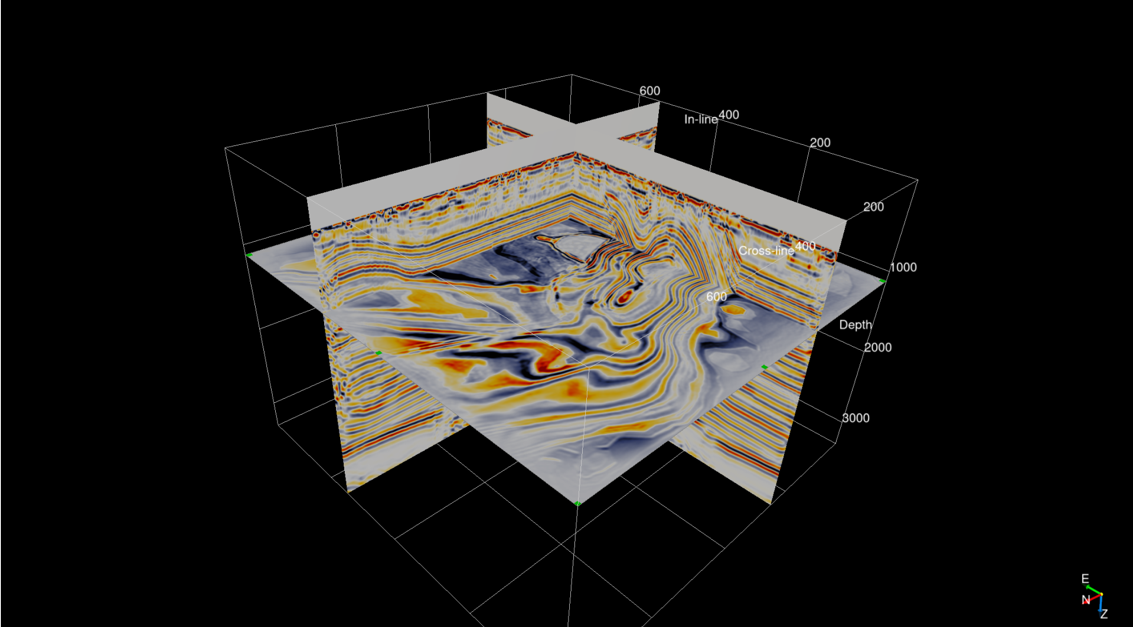
\includegraphics[width=0.500\hsize]{./Figures/OverTTI1.png}}
\subfloat[]{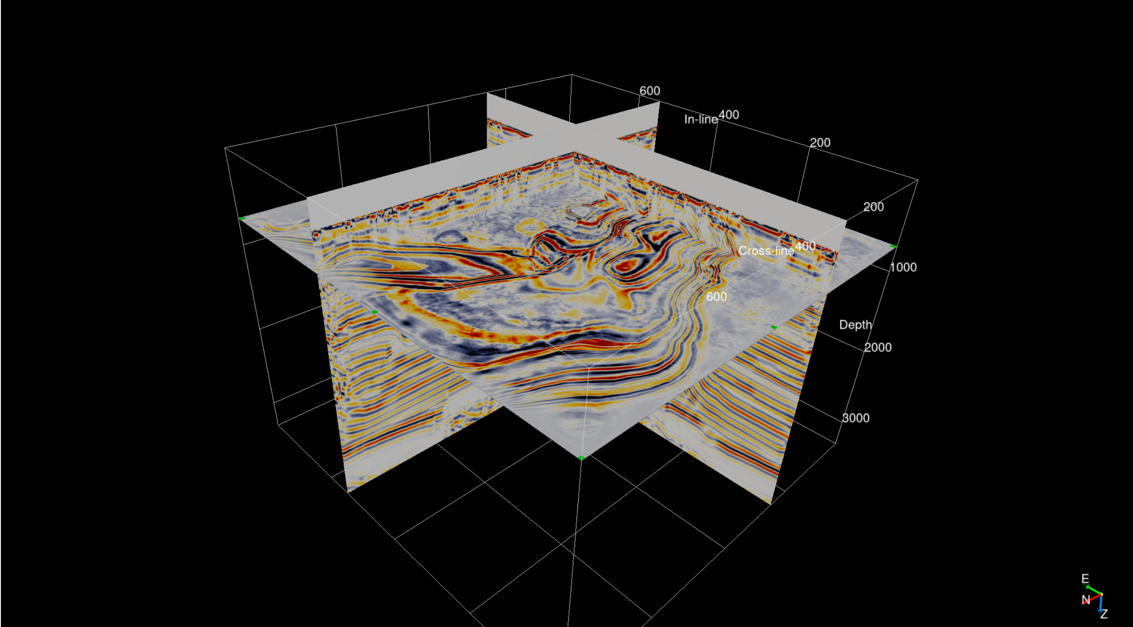
\includegraphics[width=0.500\hsize]{./Figures/OverTTI2.png}}
\\
\subfloat[]{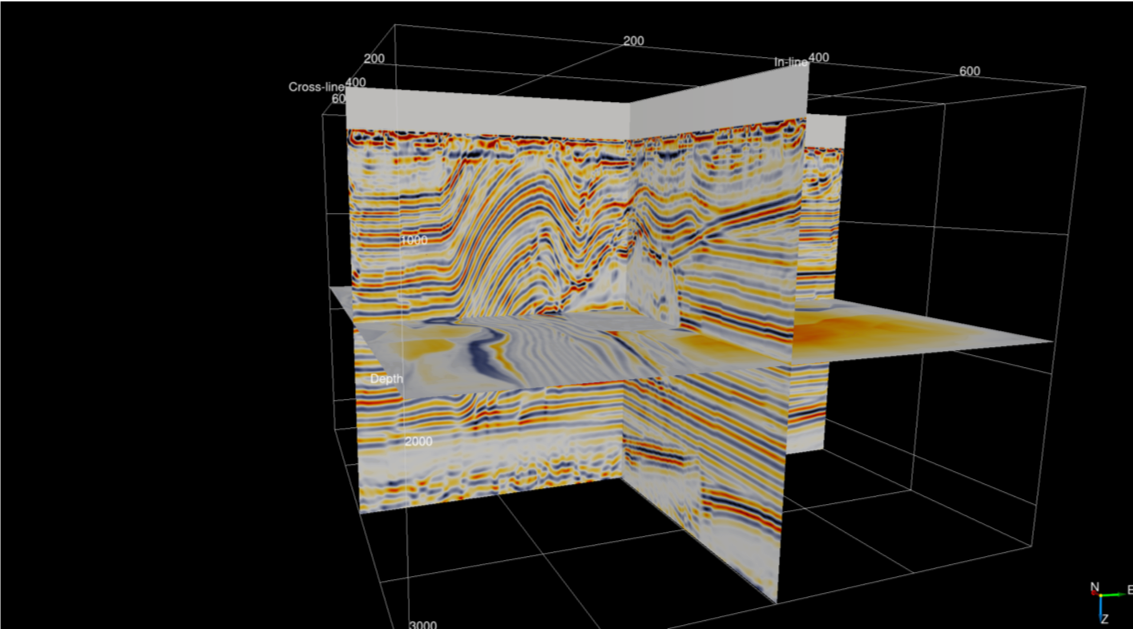
\includegraphics[width=0.500\hsize]{./Figures/OverTTI3.png}}
\subfloat[]{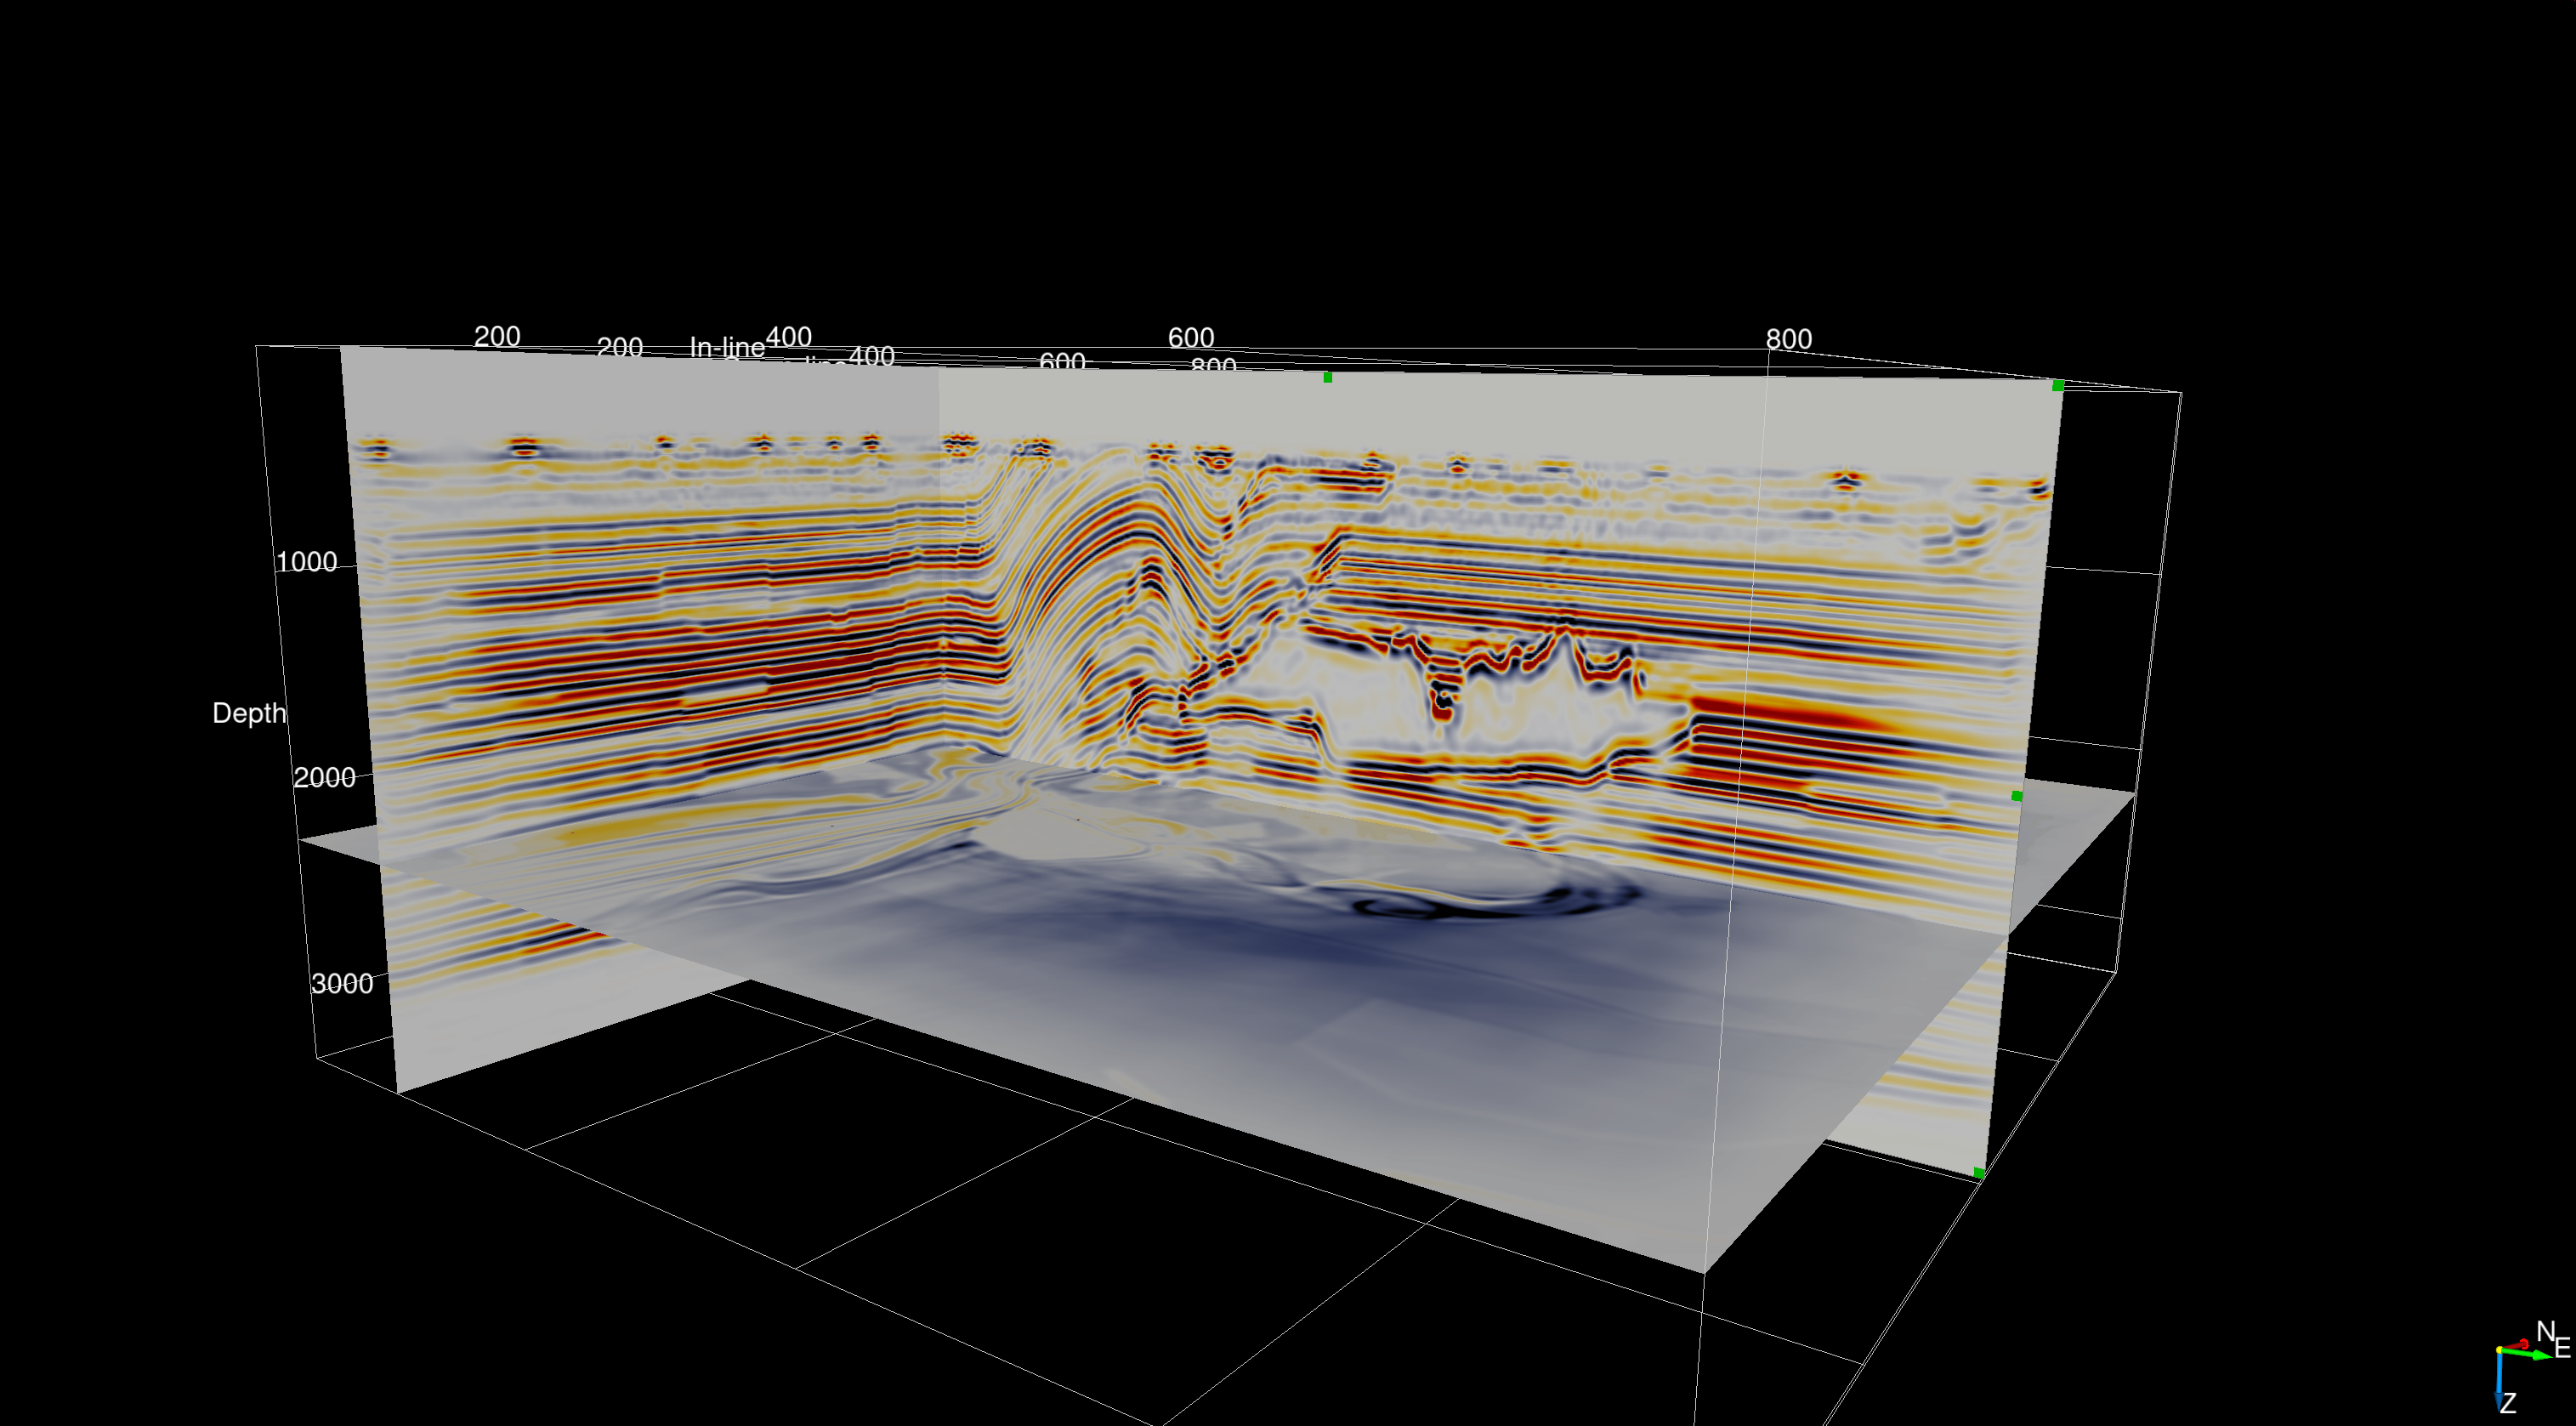
\includegraphics[width=0.500\hsize]{./Figures/OverTTI4.png}}
\caption{3D TTI imaging on a custom made model.}\label{OverTTI}
\end{figure*}

\cite{witte2019TPDedas} fully describes the serverless implementation
of seismic inverse problems, including iterative algorithms for
least-square minimization problems (LSRTM). The 3D anisotropic imaging
results were presented as part of a keynote presentation at the EAGE HPC
workshop in October 2019 \cite{herrmann2019EAGEHPCaii} and at the Rice
O\&G HPC workshop \cite{witte2019RHPCssi} where we focused on the
serverless implementation of seismic inversion algorithms in the Cloud.
This work illustrates the flexibility and portability of Devito, as we
were able to easily port a code only tested and developed on local
hardware to the Cloud, with only minor adjustments. This portability
included the possibility to run MPI-based code for domain decomposition
in the Cloud, after developing it on a desktop computer. Our experiments
are reproducible using the instructions in a public repository
\href{https://github.com/slimgroup/Azure2019}{AzureTTI}, which contains,
among the other things, the Dockerfiles and Azure
\href{https://batch-shipyard.readthedocs.io}{batch-shipyard} setup. This
example can also easily ber un on a traditional HPC cluster environment
using for exaple \href{https://github.com/slimgroup/JUDI.jl}{JUDI} or
Dask \cite{dask} for parallelization over sources.

\section{Elastic modelling}\label{elastic-modelling}

While the subsurface image in the previous Section is obtained with
anisotropic propagators capable of mimicing the real physics, in order
to model both the kinematics and the amplitudes correctly elastic
propagators are required. These propagators are for example extremely
important for global seismology, as the Shear surface waves (component
ignored in TTI) are the most hazardous ones. In this section, we exploit
the tensor algebra language introduced in
\href{https://github.com/devitocodes/devito}{Devito} v4.0 to express
elastic waves in a compact and elegant notation.

The elastic isotropic wave-equation, parametrized by the Lamé parameters
$\lambda, \mu$ and the density $\rho$ reads:
%
\begin{equation}
\begin{aligned}
&\frac{1}{\rho}\frac{dv}{dt} = \nabla . \tau \\
&\frac{d \tau}{dt} = \lambda \mathrm{tr}(\nabla v) \mathbf{I}  + \mu (\nabla v + (\nabla v)^T)
\end{aligned}
\label{elas1}
\end{equation}
%
 where $v$ is a vector valued function with one component per cartesian
direction:
%
\begin{equation}
\begin{split}
v =  \begin{bmatrix} v_x(t, x, y) \\ v_y(t, x, y)) \end{bmatrix}
\end{split}
\label{partvel}
\end{equation}
%
 and the stress $\tau$ is a symmetric second-order tensor-valued
function:
%
\begin{equation}
\begin{aligned}
    \tau = \begin{bmatrix}\tau_{xx}(t, x, y) & \tau_{xy}(t, x, y)\\\tau_{xy}t, x, y) & \tau_{yy}(t, x, y)\end{bmatrix}.
\end{aligned}
\label{stress}
\end{equation}
%
 The discretization of such a set of coupled PDEs requires five
equations in two dimensions (two equations for the particle velocity and
three for stress) and nine equations in three dimensions (three particle
velocities and six stress equations). However, the mathematical
definition only requires two coupled vector/tensor-valued equations for
any number of dimensions.

\subsection{Tensor algebra language}\label{tensor-algebra-language}

We have augmented the
\href{https://github.com/devitocodes/devito}{Devito} language with
tensorial objects to enable a straightforward -- and at the same time
mathematically rigorous -- definition of high-dimensional PDEs, such as
the elastic wave-equation in Equation~\ref{elas1}. This effort was
inspired by \cite{ufl}, a functional language for finite element
methods.

The extended \href{https://github.com/devitocodes/devito}{Devito}
language introduces two new types, \texttt{VectorFunction} (and
\texttt{VectorTimeFunction}) for vectorial objects such as the particle
velocity, and \texttt{TensorFunction} (and \texttt{TensorTimeFunction})
for second-order tensor objects (matrices) such as the stress. These new
objects are constructed the exact same way as the scalar
\texttt{Function} objects. They also automatically implement staggered
grid and staggered finite-differences with the possibility of half-node
averaging. Each component of a tensorial object -- a (scalar)
\href{https://github.com/devitocodes/devito}{Devito} \texttt{Function}
-- is accessible via conventional vector notation (i.e.
\texttt{v{[}0{]},\phantom{\ }t{[}0,1{]},....}).

With this extended language, the elastic wave-equation can be defined in
only four lines as follows:

\begin{Shaded}
\begin{Highlighting}[]
\NormalTok{v = VectorTimeFunction(name=}\StringTok{'v'}\NormalTok{, grid=model.grid, space_order=so, time_order=}\DecValTok{1}\NormalTok{)}
\NormalTok{tau = TensorTimeFunction(name=}\StringTok{'t'}\NormalTok{, grid=model.grid, space_order=so, time_order=}\DecValTok{1}\NormalTok{)}

\NormalTok{u_v = Eq(v.forward, model.damp * (v + s/rho*div(tau)))}
\NormalTok{u_t = Eq(tau.forward,  model.damp *  (tau + s * (l * diag(div(v.forward)) + mu * (grad(v.forward) + grad(v.forward).T))))}
\end{Highlighting}
\end{Shaded}

The \texttt{SymPy} expressions created by these commands can be
displayed with \texttt{sympy.pprint} as shown in
Figure~\ref{PrettyElas}. This representation reflects perfectly the
mathematics while still providing computational portability and
efficiency through the
\href{https://github.com/devitocodes/devito}{Devito} compiler. The
complete generated code for the elastic wave-equation with and without
MPI is made available at
\href{https://github.com/mloubout/SC20Paper/tree/master/gencode}{CodeSample}
in \texttt{elastic-so8.c} and \texttt{elastic-so8-mpi.c}.

\begin{figure*}
\centering
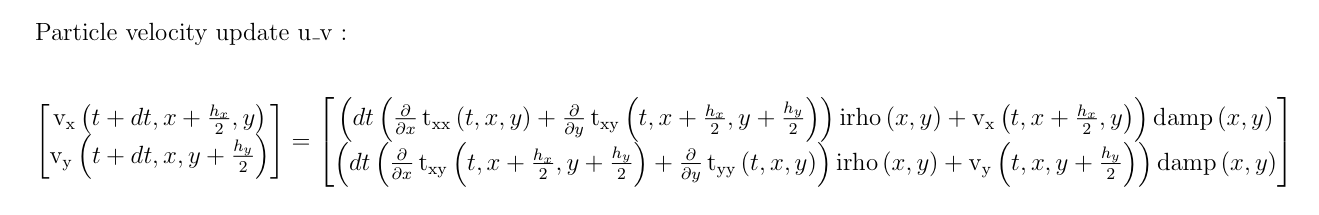
\includegraphics[width=1.000\hsize]{./Figures/vel_symb.png}
\caption{Update stencil for the particle velocity. The stencil for
updating the stress component is left out for readability, as the
equation does not fit onto a single page. However, it can be found in
the \href{https://github.com/devitocodes/devito}{Devito} tutorial on
elastic modelling on github.}\label{PrettyElas}
\end{figure*}

\subsection{2D example}\label{d-example}

We show the elastic particle velocity and stress for a broadly
recognized 2D synthetic model, the elastic
Marmousi-ii\cite{versteeg927, marmouelas} model. The wavefields are
shown on Figure~\ref{ElasWf} and its corresponding elastic shot records
are displayed in Figure~\ref{ElasShot}. Thes two figures show that the
wavefield is as expected purely acoustic in the water layer
(\texttt{t\_\{xy\}=0}) and transition perfectly at the ocean bottom to
an elastic wavefield. We can also clearly see the Shear wave wavefront
in the subsurface (around 1km depth). Thes two plots show that we
effectively solve the elastic wave-equation with an high-level
mathematical definition of the PDE that abstracts away all the
computational technicalities such as staggered grid analysis. The shot
records in Figure~\ref{ElasShot} also match the original data generated
by the creator of the elastic model in \cite{marmouelas}.

\begin{figure*}
\centering
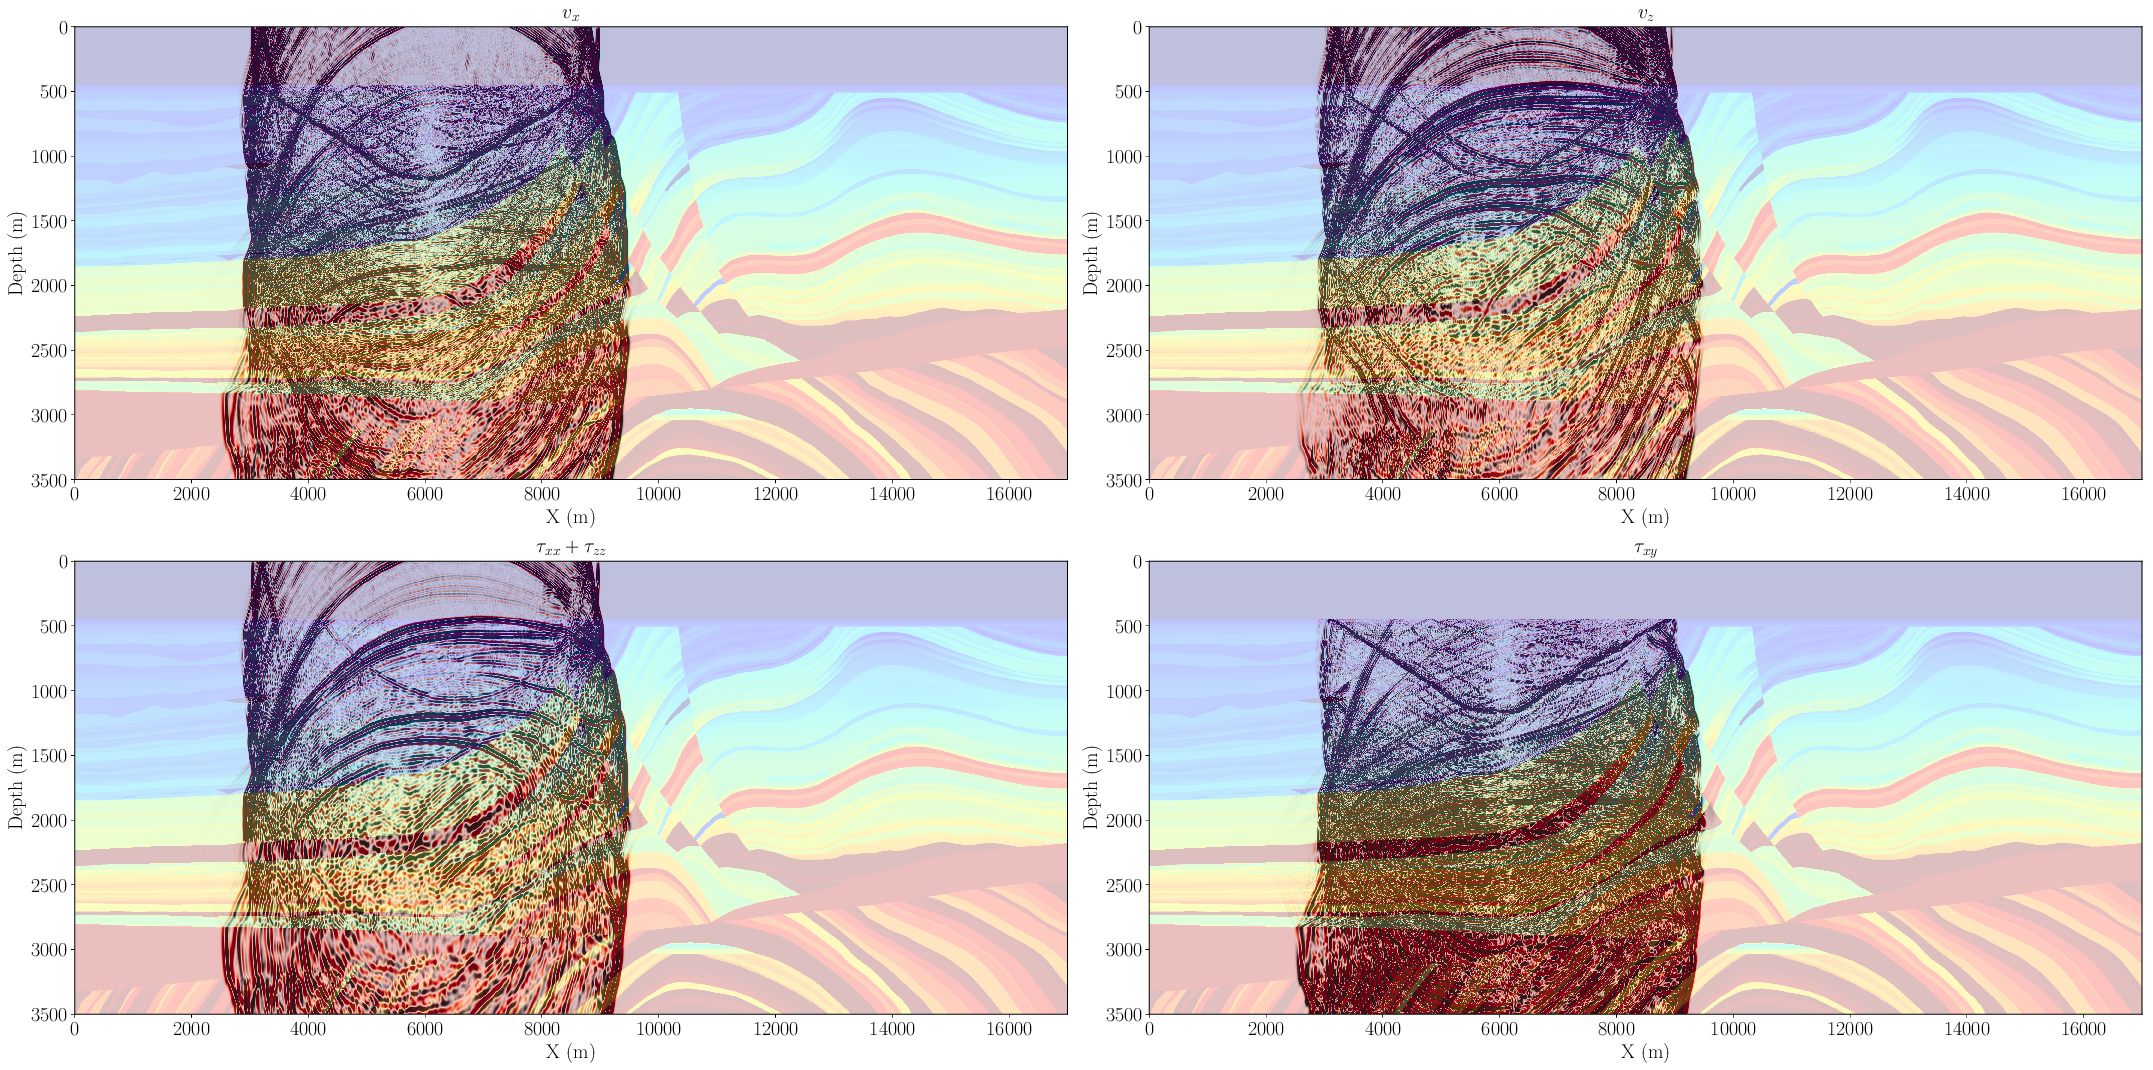
\includegraphics[width=1.000\hsize]{./Figures/marmou_snap.png}
\caption{Particle velocities and stress at time $t=3\text{s}$ for a
source at 10m depth and \texttt{x=5\textbackslash{}text\{km\}} in the
marmousi-ii model.}\label{ElasWf}
\end{figure*}

\begin{figure*}
\centering
\captionsetup[subfigure]{labelformat=empty}
\subfloat[]{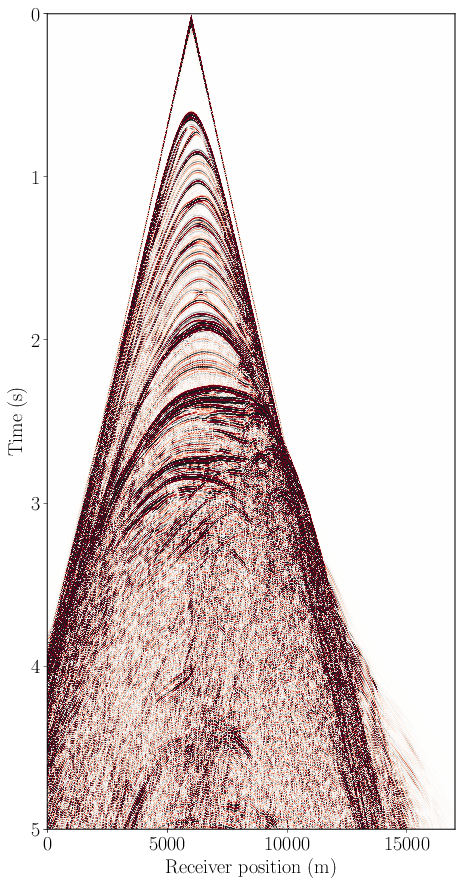
\includegraphics[width=0.300\hsize]{./Figures/pressure_marmou.png}}
\subfloat[]{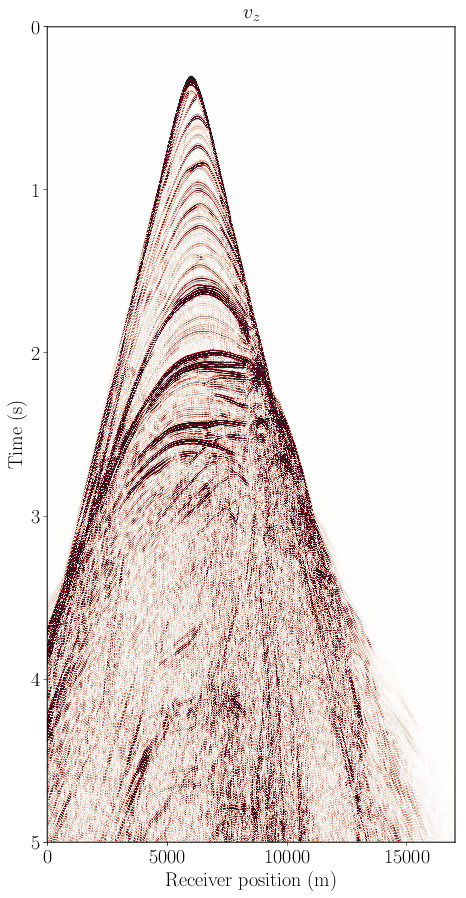
\includegraphics[width=0.300\hsize]{./Figures/vz_marmou.png}}
\subfloat[]{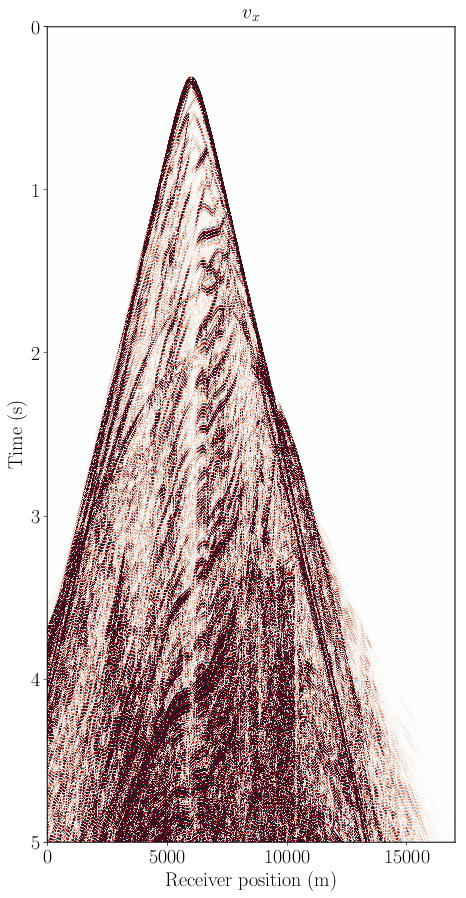
\includegraphics[width=0.300\hsize]{./Figures/vx_marmou.png}}
\caption{Seismic shot record for 5sec of modelling. \texttt{a} is the
pressure (trace of stress tensor) at the surface (5m depth), \texttt{b}
is the vertical particle velocity and \texttt{c} is the horizontal
particle velocity at the ocean bottom (450m depth).}\label{ElasShot}
\end{figure*}

\subsection{3D proof of concept}\label{d-proof-of-concept}

Finally, we modelled three dimensional elastic data in the Cloud to
demonstrate the scalability of
\href{https://github.com/devitocodes/devito}{Devito} to cluster-size
problems in the Cloud. The model we chose mimics the reference model in
geophysics known as the SEAM model \cite{fehler2011seam} that is a
three dimensional extreme-scale synthetic representation of the
subsurface. The physical dimension of the model are
\texttt{45kmx35kmx15km} then discretized with a grid spacing of
\texttt{20mx20mx10m} that led to a computational grid of
\texttt{2250x1750x1500} grid points (5.9 billion grid points). One of
the main challenges of elastic modelling is the extreme memory cost due
to the number of wavefield. For a three dimensional propagator, a
minimum of 21 fields need to be stored:

\begin{itemize}
\itemsep1pt\parskip0pt\parsep0pt
\item
  Three particle velocities with two time steps (\texttt{v.forward} and
  \texttt{v})
\item
  Six stress with two time steps (\texttt{tau.forward} and \texttt{tau})
\item
  Three model parameters \texttt{lamda}, \texttt{mu} and \texttt{rho}
\end{itemize}

These 21 fields, with the grid we just describe, leads to a minimum of
461Gb of memory for modelling only. For this experiment, we obtained
access to small HPC VM on azure called \texttt{Standard\_H16r} that are
16 cores Intel Xeon E5 2667 v3 with no hyperthreading and used 32 nodes
for a single source experiment (we solved a single wave-equation). We
used a 12th order discretization that leads to 2.8TFLOP/time-step to be
computed for this model and propagated the elastic wave for 16 seconds
(23000 time steps). The modelling ran in 16 hours which converts to
1.1TFLOP/s. While these number may seem low, the elastic kernel is
extremely memory bound, while the TTI kernel is nearly compute bound
(see rooflines in \cite{louboutin2016ppf, devito-api, devito-compiler})
making it more computationally efficient, in particular in combination
with MPI. Future work with involve working on the InfiniBand enabled and
true HPC VM on azure to achieve Cloud performance on par with state of
the art Cluster performance. From the performance obtained in this
experiement, and assuming a fairly standard setup of 5000 independent
source experiements, computing a synthetic dataset would require 322
EFLOP to be computed (23k time-steps x 2.8TFLOP/time-step x 500
sources), or using the full scalability and computing all sources in
parallel would lead to 5.5PFLOP/s from our single source experiement
result.

\section{Performance comparison with other
codes}\label{performance-comparison-with-other-codes}

Because earlier performance benchmark focuse mainly on roofline model
analysis, we also compared the runtime of
\href{https://github.com/devitocodes/devito}{Devito} with a reference
open source hand-coded propagator in collaboration with its author for
compeleteness. This propagator, described in \cite{thorbecke} is a
state of the art elastic kernel (Equation~\ref{elas1}). For a fair
comparison, we ensure, in collaboration with the author of
\href{https://github.com/JanThorbecke/OpenSource.git}{fdelmodc} that the
physical and computational settings were identical. The setting were the
following:

\begin{itemize}
\itemsep1pt\parskip0pt\parsep0pt
\item
  2001 by 1001 physical grid points.
\item
  200 grid points of dampening layer (absorbing layer \cite{cerjan}) on
  all four sides (total of 2401x1401 computational grid points).
\item
  10001 time steps.
\item
  Single point source, 2001 receivers.
\item
  Same compiler (gcc/icc) to compile
  \href{https://github.com/JanThorbecke/OpenSource.git}{fdelmodc} and
  run Devito.
\item
  Intel(R) Xeon(R) CPU E3-1270 v6 @ 3.8GHz.
\item
  Single socket, four physical cores, four physical threads, thread
  pinning to cores and hyperthreading off.
\end{itemize}

The runtime obtained for this problem for both propagators were
identical with less than one percent of difference. This similar runtime
were obtained both with the Intel compiler and the GNU compiler and we
ran the experiment with a fourth order and a sixth order discretization.
The kernels were executed five time each to ensure consistency between
the results and we consistently obtained similar runtimes. This
comparison illustrates the performance achieved with
\href{https://github.com/devitocodes/devito}{Devito} is at least on par
with hand-coded propagators. Considering we do not take adantage of the
\href{https://github.com/devitocodes/devito}{Devito} compiler full
capabilities in the two dimensional case, we are confident that the
generated code will be at least on par with hand-coded version for three
dimensional probalems and this comparison will be part of future work.

\section{Conclusions}\label{conclusions}

The transition from academic size problems, such as the two-dimensional
acoustic wave-equation, to real-world application can be challenging in
particular when attempted as an afterthought. In this work, we showed
that thanks to design principles that aimed at this type of application
from the beginning, \href{https://github.com/devitocodes/devito}{Devito}
provides the scalability necessary. First, we showed that we provide a
high-level interface not only for simple scalar equations but for
coupled PDEs and allow the expression of non-trivial differential
operators in a simple and concise way. Second and most importantly, we
demonstrated that the compiler enables large-scale with state-of-the art
computational performance and programming paradigm. The single-node
performance is on par with hand-coded codes while providing the
flexibility from the symbolic interface, and multi-node parallelism is
integrated in the compiler and interface in a conservative way. Finally,
we demonstrated that our abstraction provides to performance portability
that enables both on-premise HPC and Cloud HPC.


\bibliography{sc20_paper}


\end{document}

